\documentclass[11pt]{beamer}
\usetheme{Madrid}
\usefonttheme{serif}

\usepackage[utf8]{inputenc}
\usepackage[spanish]{babel}
\usepackage[T1]{fontenc}

\usepackage{amsmath}
\usepackage{amsfonts}
\usepackage{amssymb}
\usepackage{graphicx}
\usepackage{booktabs}
\usepackage{array}
\usepackage{tabularx}
\usepackage{ragged2e}
\usepackage{hyperref}
\usepackage{xurl}
\usepackage{xcolor}

\Urlmuskip=0mu plus 1mu

\newcommand{\ulorange}[1]{\textcolor{orange}{\underline{\textcolor{black}{#1}}}}
\newcommand{\ulred}[1]{\textcolor{red}{\underline{\textcolor{black}{#1}}}}

\setbeamertemplate{navigation symbols}{}
\setbeamertemplate{caption}[numbered]

% --- Metadatos ----------------------------------------------------------

\author{Luis Miguel Muñoz Barón}
% Título de portada más breve; el subtítulo conserva el marco de datos.
\title[TEA en adultos / AQ-10]{%
  Modelo de clasificación de TEA en adultos
  basado en el cuestionario AQ-10
}
\subtitle{Conjunto UCI \emph{Adult Autism Screening} (F.~Thabtah, 2017)}
\date{2026}

\institute[]{%
  Diplomado en Inteligencia Artificial Aplicada 2026\\[0.2em]
  IPICYT
}

\titlegraphic{%
  \IfFileExists{imagens/fciencias_escudo.png}{%
    \centering
    \includegraphics[height=2cm]{imagens/fciencias_escudo.png}
  }{}%
}

\bibliographystyle{apalike}

% --- Columna descriptiva alineada como en documento largo ---------------
\newcolumntype{L}{>{\RaggedRight\arraybackslash}X}

\begin{document}

\begin{frame}
  \titlepage
\end{frame}

% -------------------------------------------------------------------------
\section{Guía de la presentación}

\begin{frame}{Índice (preguntas analíticas)}
  \begin{itemize}
    \setlength{\itemsep}{0.35em}
    \item \textbf{Ítems:} contribución diferencial de A1--A10 frente a esquema de puntuación fija.
    \item \textbf{Subgrupos:} perfiles de respondientes y patrones en las respuestas.
    \item \textbf{Forma corta:} subconjuntos de ítems con desempeño comparable (p.\,ej.\ AUROC/F1).
    \item \textbf{Regla \emph{vs.} modelo:} coherencia y desacuerdos con el umbral tipo \texttt{result $>$ 6}.
    \item \textbf{Equidad:} errores y métricas en subgrupos (sexo, edad, región) con soporte muestral suficiente.
  \end{itemize}
  \vspace{0.4em}
  {\footnotesize\color{gray} Orden sugerido en el cuaderno: base e importancia $\rightarrow$ regla fija $\rightarrow$ reducción de ítems $\rightarrow$ clustering $\rightarrow$ equidad.}
\end{frame}

% -------------------------------------------------------------------------
\section{Plantamiento y motivación del estudio}

\begin{frame}{El desafío del diagnóstico y el tamizaje}
  El TEA implica desafíos en comunicación, interacción social y patrones de conducta. El diagnóstico formal en clínica es largo y costoso; se estima $\sim$1.5\,\% de prevalencia global y subdiagnóstico frecuente.\\[0.45em]
  Herramientas como ADI y ADOS son referencia, pero generan cuellos de botella: muchas personas no acceden a evaluación oportuna.\\[0.45em]
  Los tamices breves y autoadministrables orientan hacia valoración especializada \emph{sin} sustituir el diagnóstico: optimizan rutas y uso de recursos clínicos.
\end{frame}

\begin{frame}{Diagnóstico en adultos y tamizaje en contexto restringido}
  En adultos, el diagnóstico suele demorarse por invisibilidad de síntomas, compensación social y poca formación en detección en edad adulta.\\[0.45em]
  En México, demoras y costos limitan el acceso; en el primer nivel faltan protocolos sistemáticos y la oferta privada se torna inaccesible.\\[0.45em]
  Instrumentos de tamizaje \textbf{no} son diagnóstico: actúan como \emph{primer filtro} para priorizar evaluación formal.
\end{frame}

\begin{frame}{Herramienta de tamizaje: Autism Spectrum Quotient-10}
  El \textbf{AQ-10} es un tamiz breve (10 ítems) para indicios de rasgos asociados al TEA en adultos; se deriva del AQ-50.\\[0.4em]
  Cada ítem se califica y produce un puntaje total; un \textbf{umbral} predefinido (p.\,ej.\ $\geq 6$) sugiere profundizar con evaluación clínica.\\[0.4em]
  Características: autoinforme, bajo costo, útil cuando el acceso a especialistas es limitado. El propósito es \textbf{identificación preliminar} y ruta a especialistas, no etiqueta clínica definitiva.
\end{frame}

% -------------------------------------------------------------------------
\section{Metodología y composición de datos}

\begin{frame}{Conjunto de datos (UCI) y enlace con \textit{ASDTests}}
  Se usa el conjunto público del \textbf{UCI Machine Learning Repository} (cribado de rasgos vinculados al TEA en adultos/otras edades), aportado por F.~Thabtah y alineado con criterios tipo DSM-5.\\[0.4em]
  Proviene de la app \textbf{\textit{ASDTests}}: cuestionarios breves, captura de metadatos y cálculo de puntaje; en este estudio se trabaja con la categoría \textbf{Adulto}.\\[0.4em]
  \footnotesize\color{gray} Ver composición y variables en el cuadro siguiente (misma lógica que en \texttt{prop.tex}).
\end{frame}

% --- Cuadro 1: misma estructura y contenido que prop.tex, desc. en ES -----
\begin{frame}{Cuadro 1. Features y correspondencia con AQ-10 (1/5)}
  \vspace{-0.2em}
  \begin{center}
    \scriptsize
    \textbf{Tabla.} \emph{Features recopiladas, descripciones y correspondencia con el cuestionario AQ-10.} (Metadatos I)
  \end{center}
  \vspace{0.2em}
  {\tiny
  \begin{tabularx}{\linewidth}{@{}l l L@{}}
    \toprule
    \textbf{Feature} & \textbf{Tipo} & \textbf{Descripción} \\
    \midrule
    Age & Número & Adultos (año); es decir, 17 años o más. \\
    Gender & String & Hombre o mujer. \\
    Ethnicity & String & Lista de etnias frecuentes (texto). \\
    Born with jaundice & Boolean (sí/no) & Indica si la persona nació con ictericia. \\
    Family member with PDD & Boolean (sí/no) & Un familiar inmediato con TDD. \\
    \bottomrule
  \end{tabularx}
  }
\end{frame}

\begin{frame}{Cuadro 1. Features y correspondencia con AQ-10 (2/5)}
  \vspace{-0.2em}
  \begin{center}
    \scriptsize
    \textbf{Tabla.} (Metadatos II y entorno)
  \end{center}
  \vspace{0.2em}
  {\tiny
  \begin{tabularx}{\linewidth}{@{}l l L@{}}
    \toprule
    \textbf{Feature} & \textbf{Tipo} & \textbf{Descripción} \\
    \midrule
    Who is completing the test & String & Padre, la persona, cuidador, personal de salud, clínica, etc. \\
    Country of residence & String & Países (texto). \\
    Used the screening app before & Boolean (sí/no) & Si ya usó la app de tamizaje. \\
    Screening method type & Entero (0,1,2,3) & 0: Toddler; 1: Child; 2: Adolescent; 3: \textbf{Adult}. Aquí solo Adult. \\
    \bottomrule
  \end{tabularx}
  }
\end{frame}

\begin{frame}{Cuadro 1. Ítems A1--A5 (3/5)}
  \vspace{-0.3em}
  \begin{center}
    \scriptsize
    \textbf{Tabla.} (Ítems binarios; texto adaptado al español, mismo enunciado que en \texttt{prop.tex})
  \end{center}
  \vspace{0.2em}
  {\tiny
  \begin{tabularx}{\linewidth}{@{}l l L@{}}
    \toprule
    \textbf{Feature} & \textbf{Tipo} & \textbf{Descripción} \\
    \midrule
    A1 & Binary (0,1) & A menudo noto sonidos leves que otros no perciben. \\
    A2 & Binary (0,1) & Suelo concentrarme más en el conjunto que en detalles pequeños. \\
    A3 & Binary (0,1) & Me resulta fácil hacer más de una cosa a la vez. \\
    A4 & Binary (0,1) & Si me interrumpen, vuelvo enseguida a lo que hacía. \\
    A5 & Binary (0,1) & Me resulta fácil ``leer entre líneas'' si alguien me habla. \\
    \bottomrule
  \end{tabularx}
  }
  \vspace{0.25em}
  \begin{center}
  {\tiny Abreviaturas en pie de tesis: PDD, ASD (véase nota al final de la serie de tablas).}
  \end{center}
\end{frame}

\begin{frame}{Cuadro 1. Ítems A6--A10 (4/5)}
  \vspace{-0.3em}
  \begin{center}
    \scriptsize
    \textbf{Tabla.} (Ítems 6--10, mismo orden que en \texttt{prop.tex})
  \end{center}
  \vspace{0.2em}
  {\tiny
  \begin{tabularx}{\linewidth}{@{}l l L@{}}
    \toprule
    \textbf{Feature} & \textbf{Tipo} & \textbf{Descripción} \\
    \midrule
    A6 & Binary (0,1) & Sé cómo notar si quien me escucha se aburre. \\
    A7 & Binary (0,1) & Al leer una historia me cuesta interpretar intenciones de personajes. \\
    A8 & Binary (0,1) & Me gusta reunir datos sobre categorías (coches, aves, trenes, plantas, etc.). \\
    A9 & Binary (0,1) & Me resulta fácil inferir qué piensa o siente alguien por su rostro. \\
    A10 & Binary (0,1) & Me cuesta interpretar intenciones ajenas. \\
    \bottomrule
  \end{tabularx}
  }
\end{frame}

\begin{frame}{Cuadro 1. Puntaje, etiqueta y nota (5/5)}
  \vspace{-0.2em}
  {\tiny
  \begin{tabularx}{\linewidth}{@{}l l L@{}}
    \toprule
    \textbf{Feature} & \textbf{Tipo} & \textbf{Descripción} \\
    \midrule
    ASD score & Entero & Puntaje con la regla del AQ-10-Adulto (cálculo automático). \\
    Class label & Boolean & Decisión según el AQ-10 Adulto: 0 (sin indicios) o 1 (con indicios de rasgos ASD). \\
    \bottomrule
  \end{tabularx}
  }
  \vspace{0.5em}
  \begin{block}{}
    \tiny
    \textbf{Nota.} TDD: trastorno generalizado del desarrollo; \textbf{ASD:} trastorno del espectro autista. Un puntaje por encima del umbral (p.\,ej.\ ${>}6$) en adultos orienta a evaluación clínica, como en el texto del trabajo escrito; el modelado con ML contrasta y explica, no reemplaza esa ruta.
  \end{block}
\end{frame}

% -------------------------------------------------------------------------
\begin{frame}{Distribuciones del conjunto de datos}
  \vspace{-0.3em}
  \begin{columns}[T]
    \begin{column}{0.49\textwidth}
      \begin{center}
        {\tiny \textbf{Distribuciones generales} (edad, puntaje, género, etnia, países, ictericia, antecedentes familiares, relación)}\\[0.3em]
        \IfFileExists{imagens/eda_overview.png}{%
          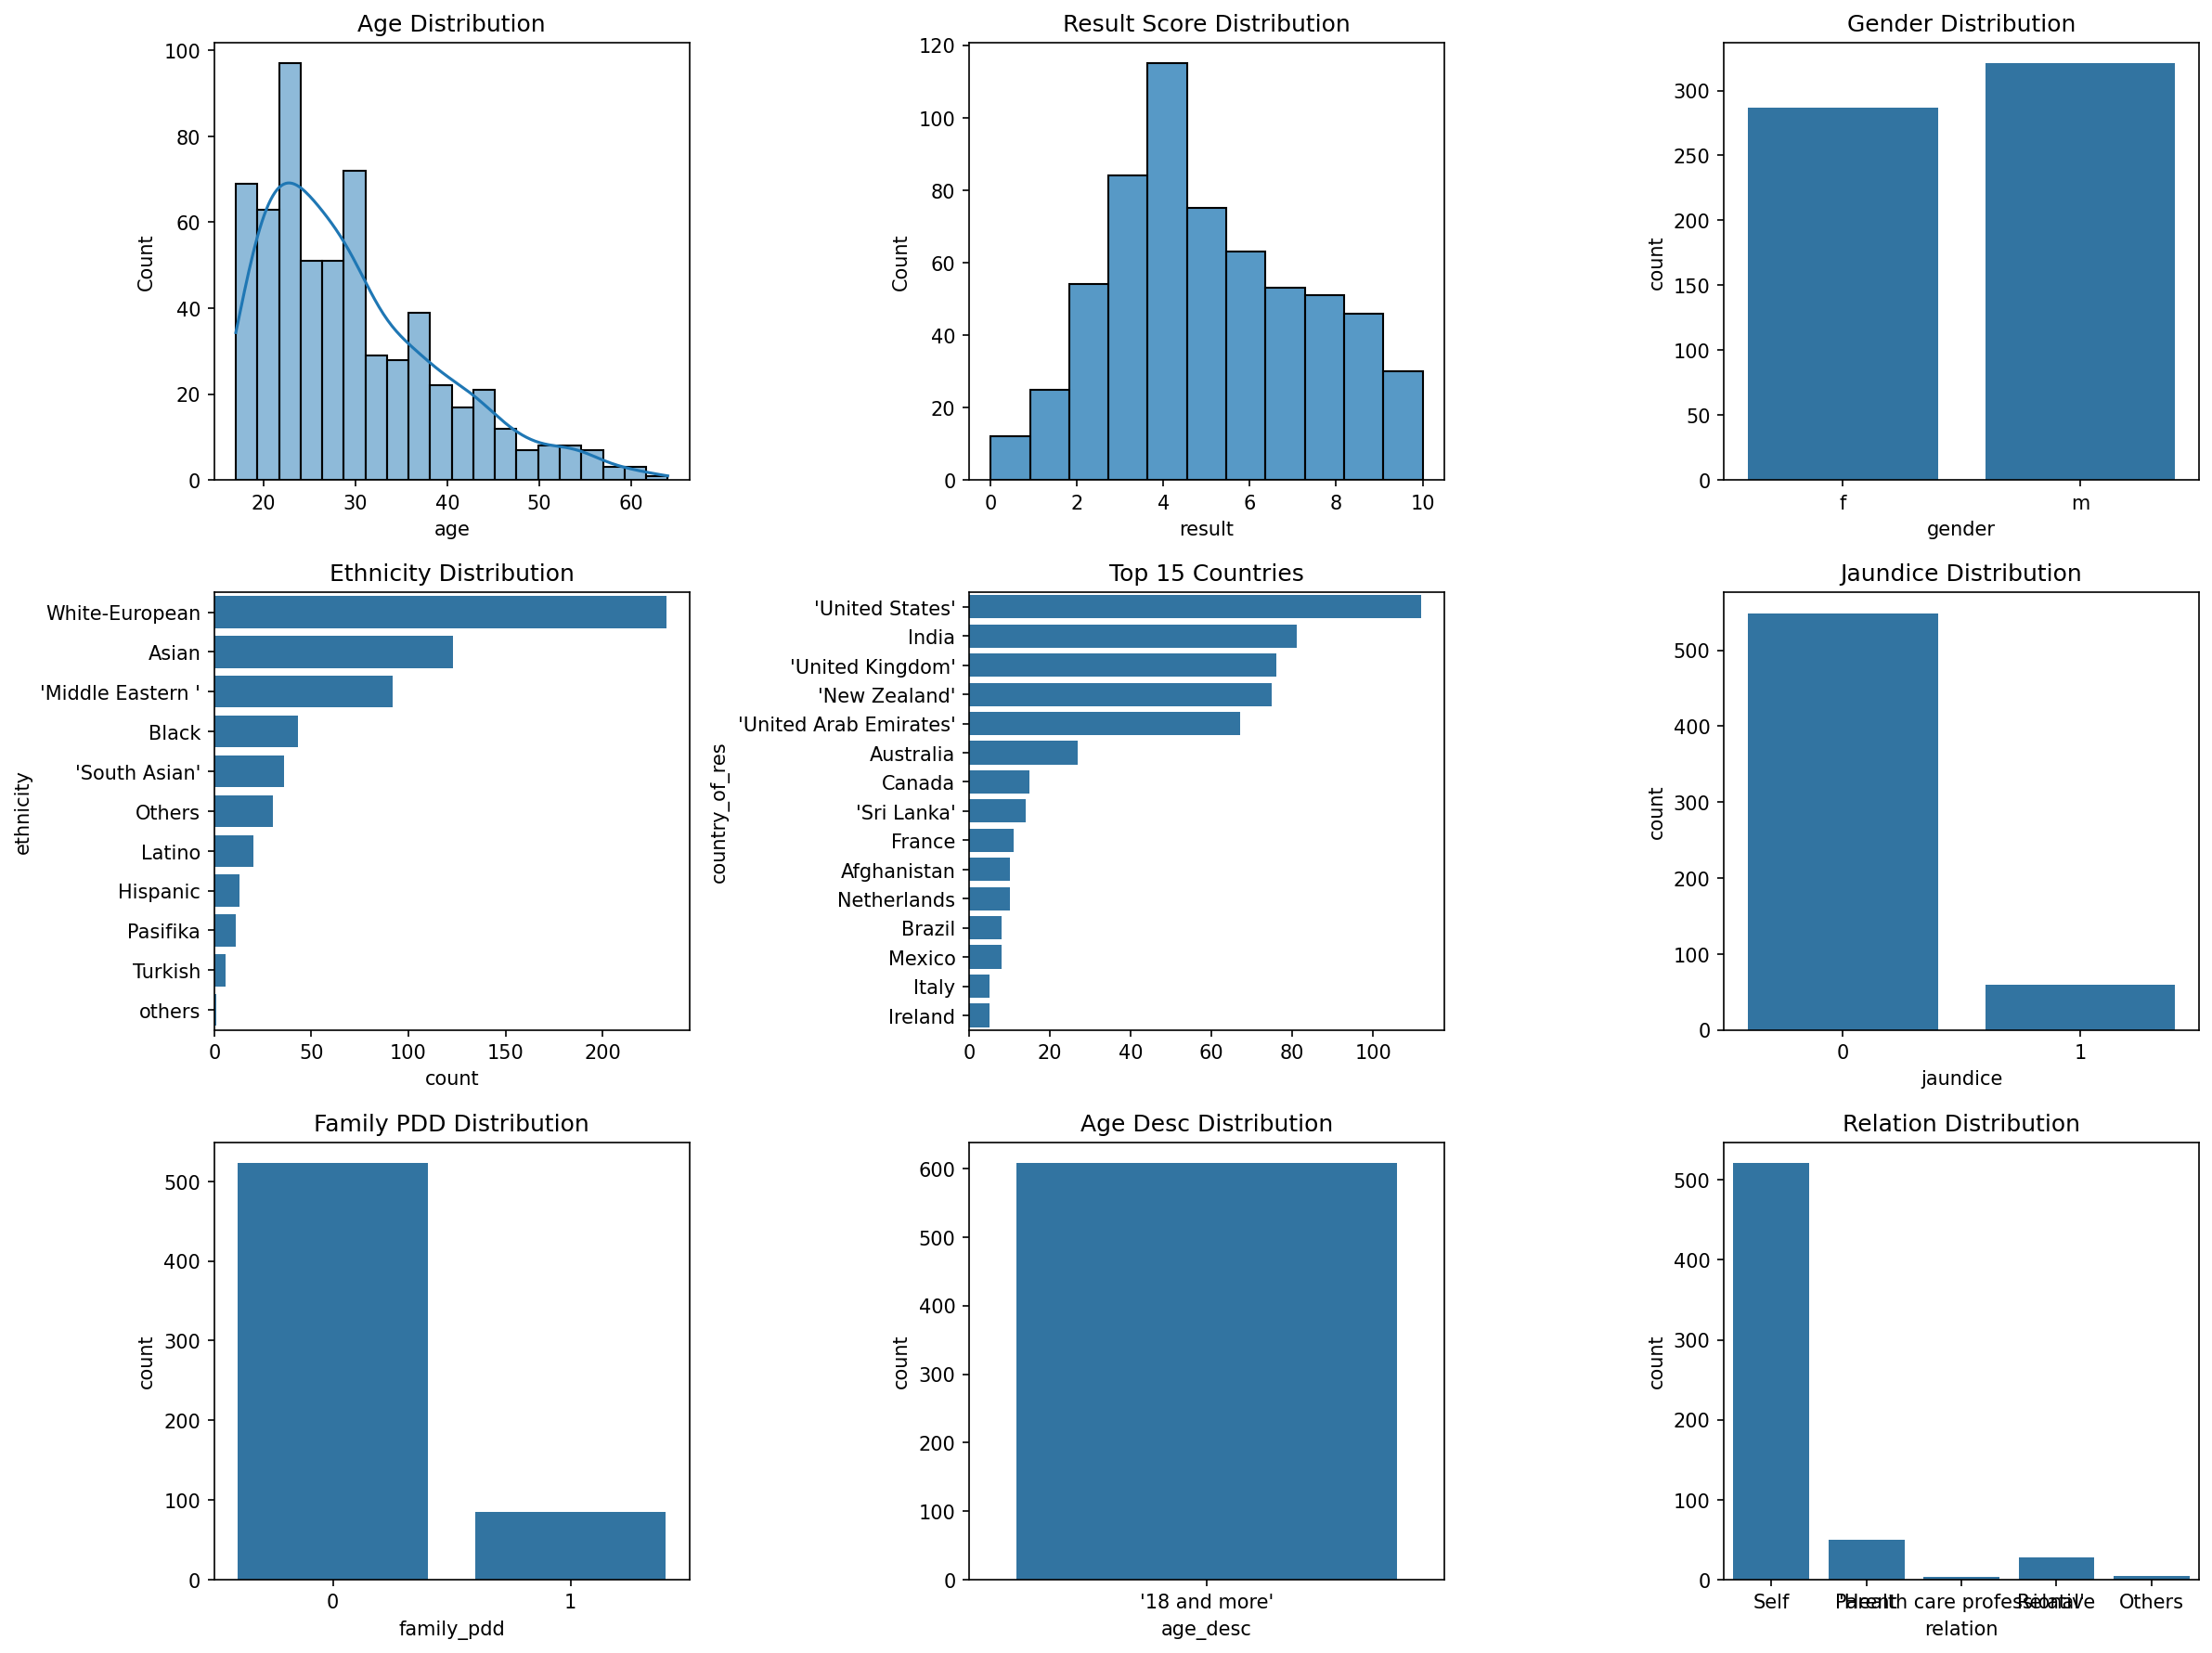
\includegraphics[width=\linewidth]{imagens/eda_overview.png}
        }{%
          \textcolor{gray}{\tiny [Ejecutar el cuaderno para generar \texttt{imagens/eda\_overview.png}]}
        }
      \end{center}
    \end{column}
    \begin{column}{0.49\textwidth}
      \begin{center}
        {\tiny \textbf{Distribuciones por clase ASD} (ASD vs.\ no-ASD por ítem, edad y puntaje)}\\[0.3em]
        \IfFileExists{imagens/eda_by_class.png}{%
          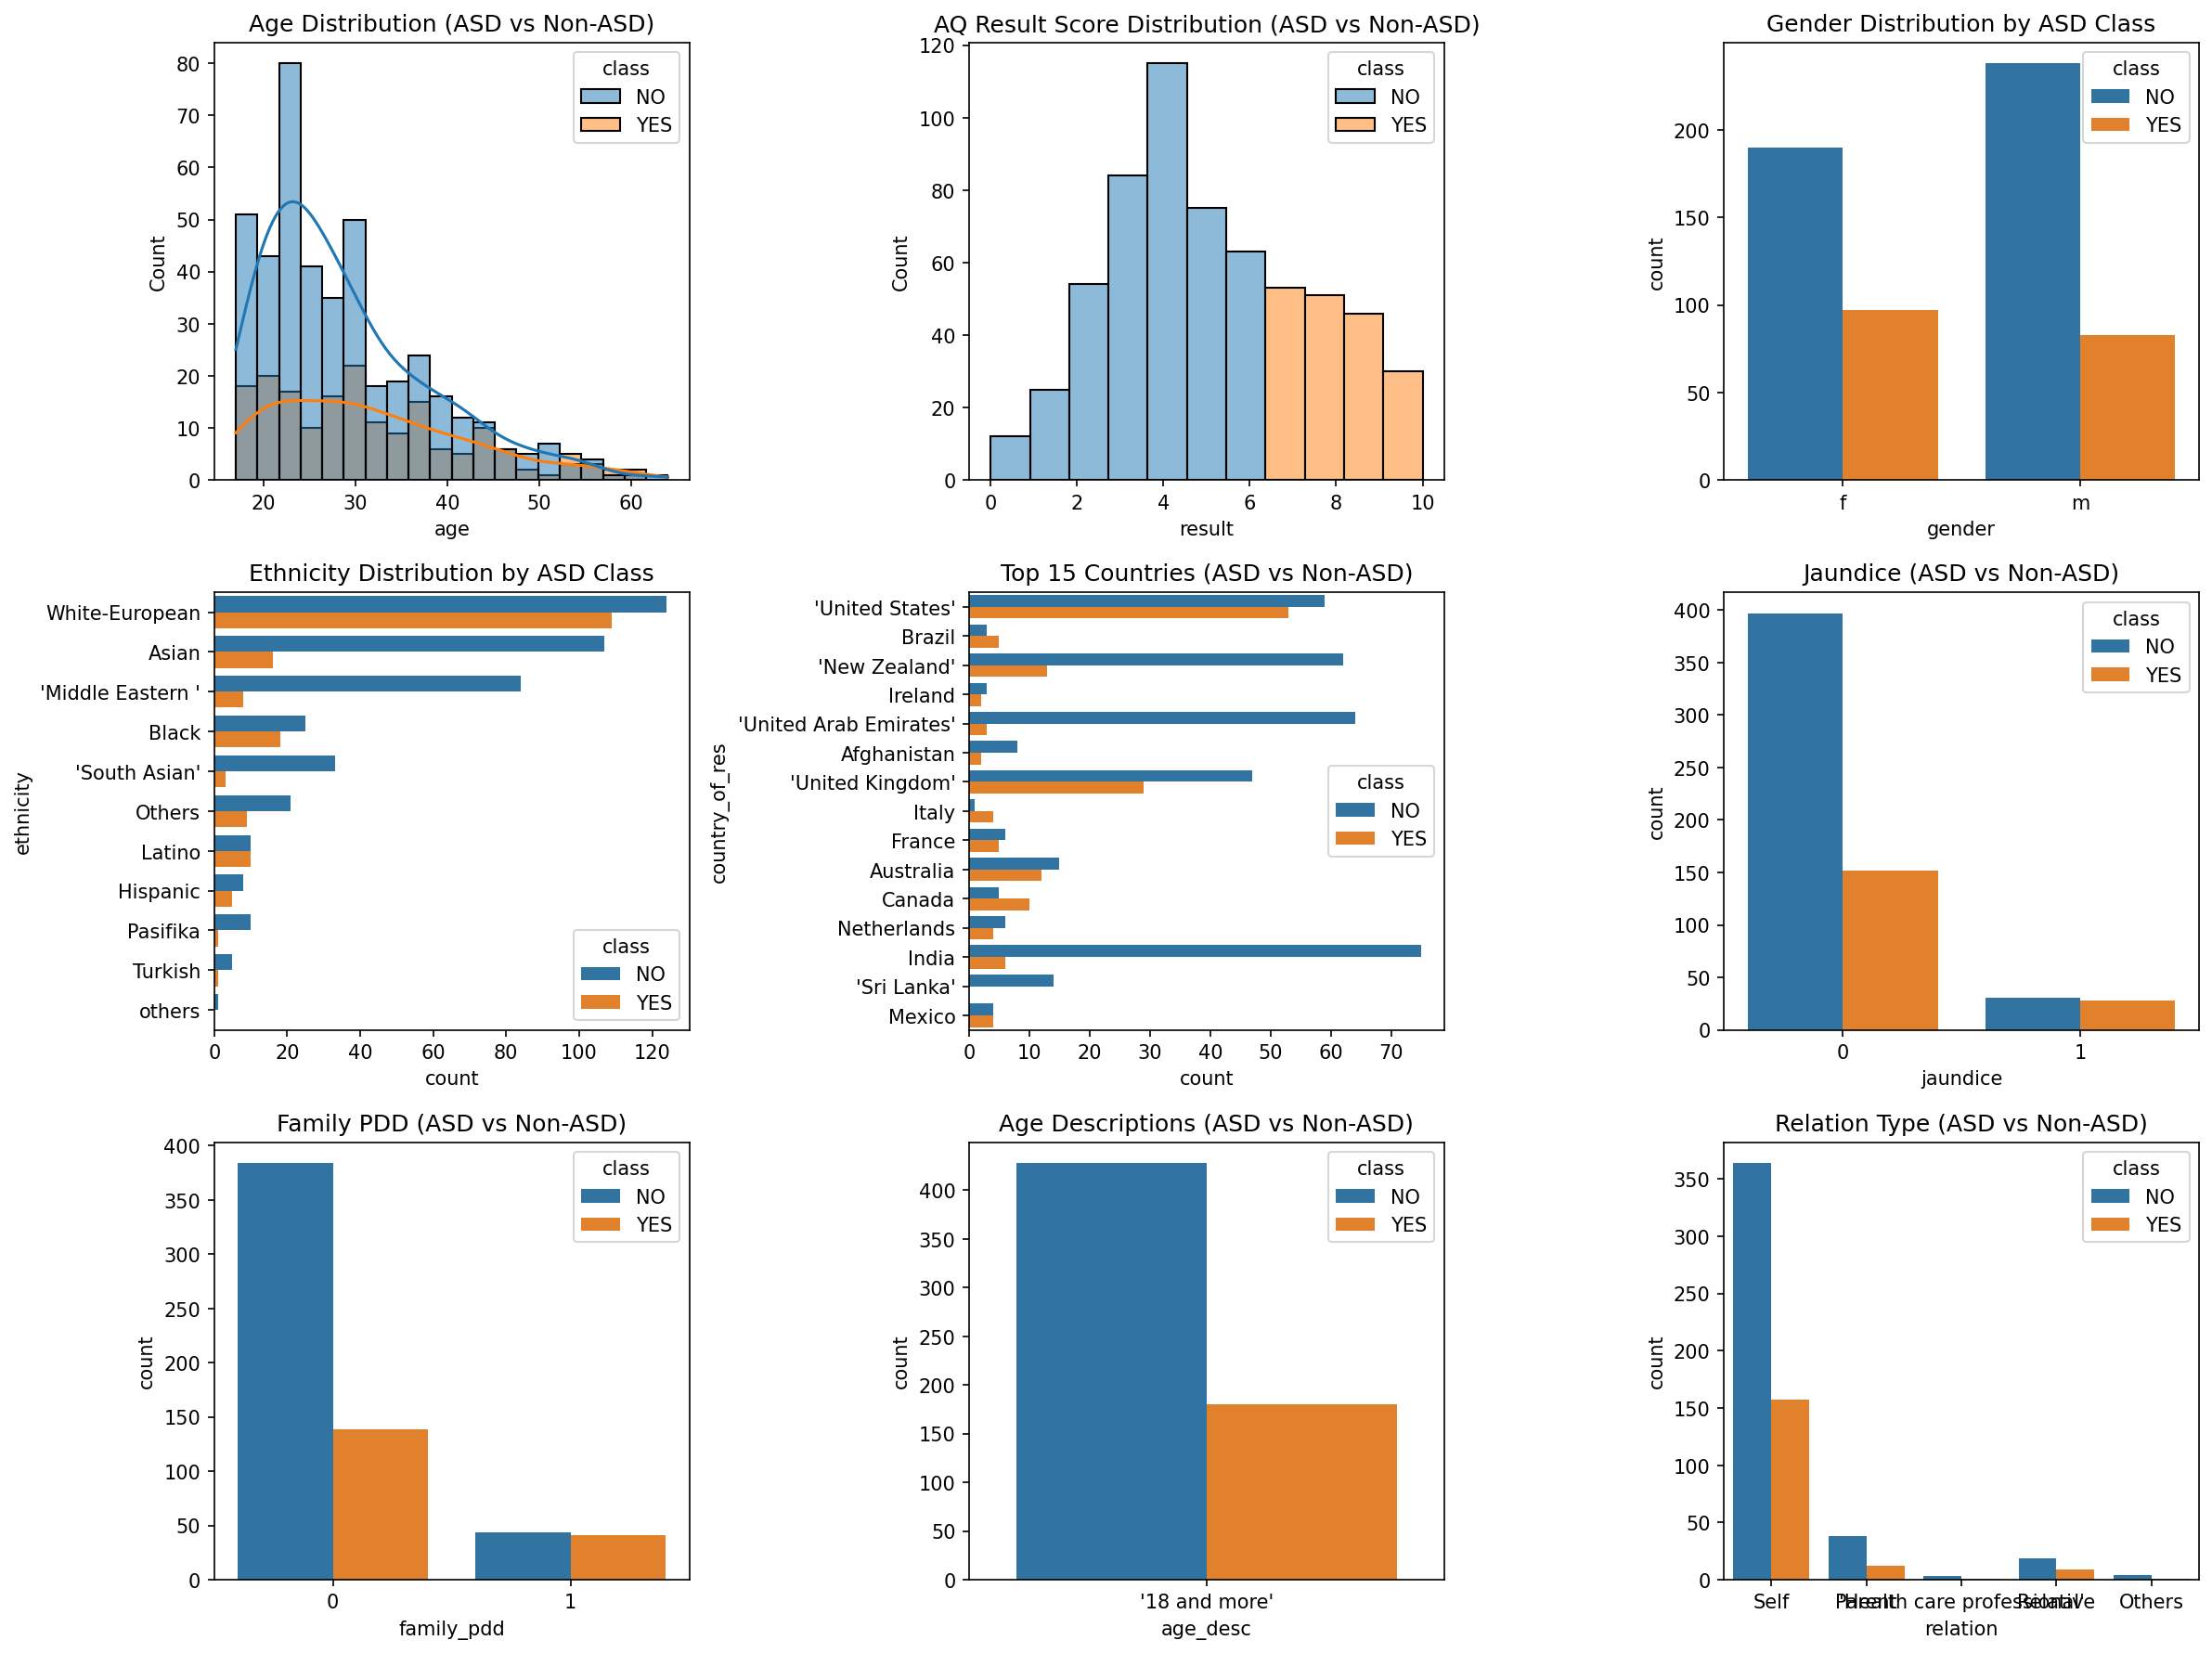
\includegraphics[width=\linewidth]{imagens/eda_by_class.png}
        }{%
          \textcolor{gray}{\tiny [Ejecutar el cuaderno para generar \texttt{imagens/eda\_by\_class.png}]}
        }
      \end{center}
    \end{column}
  \end{columns}
\end{frame}

% -------------------------------------------------------------------------
\section{Objetivos, preguntas y resultados previstos}

\begin{frame}{Objetivos y carácter del estudio}
  \begin{itemize}
    \setlength{\itemsep}{0.3em}
    \item \textbf{Metodológico--analítico:} expresividad del AQ-10 con modelos \emph{interpretables}: contribución por ítem, redundancias, patrones más allá de umbrales fijos.
    \item \textbf{Clínico--operativo:} apoyo al tamizaje preliminar, mejor uso de recursos, \textbf{sin} sustituir diagnóstico experto.
  \end{itemize}
  \vspace{0.4em}
  {\footnotesize La literatura con este conjunto aún es limitada: enfoque \textbf{exploratorio} y comparación de modelos, como en el planteamiento de \texttt{prop.tex}.}
\end{frame}

\begin{frame}{Preguntas de investigación (I)}
  \begin{enumerate}
    \setlength{\itemsep}{0.25em}
    \item ¿Aportan modelos interpretables información extra al puntuar el AQ-10 con pesos similares y umbral fijo?
    \item ¿Hay ítems más informativos o redundantes desde la evidencia de datos?
    \item ¿Existen perfiles o patrones latentes más allá del puntaje total?
  \end{enumerate}
\end{frame}

\begin{frame}{Preguntas de investigación (II)}
  \begin{enumerate}
    \setcounter{enumi}{3}
    \setlength{\itemsep}{0.25em}
    \item ¿Puede estimarse de forma aceptable el riesgo o la probabilidad de tamizaje con un subconjunto de ítems?
    \item ¿Difieren el comportamiento o la importancia de los ítems entre subgrupos (sexo, edad, región)?
    \item ¿Qué ventajas y límites tienen modelos explicables frente a reglas fijas en claridad y apoyo a decisiones iniciales?
  \end{enumerate}
\end{frame}

\begin{frame}{Metodología (resumen alineado con el texto del trabajo)}
  \begin{enumerate}
    \setlength{\itemsep}{0.2em}
    \footnotesize
    \item EDA: distribución de ítems, correlaciones, redundancias.
    \item Partición \textbf{estratificada} en entrenamiento, validación y prueba.
    \item Modelos interpretables: regresión logística, árboles, \textbf{Random Forest} y línea base con regla de puntuación.
    \item Métricas: sensibilidad, especificidad, AUC-ROC; casos límite.
    \item Interpretación: coeficientes, importancia, SHAP (global/local).
    \item Métodos no supervisados: clustering, factorial o PCA, según celdas del cuaderno.
    \item Evaluación de \textbf{reducción de ítems} en desempeño y estabilidad.
  \end{enumerate}
\end{frame}

\begin{frame}{Random Forest: implementación}
  \begin{columns}[T]
    \begin{column}{0.52\textwidth}
      \textbf{Pipeline de preprocesamiento}
      \begin{itemize}
        \setlength{\itemsep}{0.2em}
        \footnotesize
        \item Escalado $z$-score para variables numéricas (ítems, edad, metadatos binarios).
        \item \emph{One-hot encoding} para variables categóricas (género, etnia, país, relación).
      \end{itemize}
      \vspace{0.4em}
      \textbf{Clasificador}
      \begin{itemize}
        \setlength{\itemsep}{0.2em}
        \footnotesize
        \item 300 árboles, profundidad máx.\ 12, \texttt{min\_samples\_leaf=2}.
        \item \texttt{class\_weight=``balanced''}: compensa la clase minoritaria (ASD).
        \item Variable objetivo: \texttt{class\_binary} (1\,=\,YES, 0\,=\,NO); \texttt{result} excluido.
      \end{itemize}
    \end{column}
    \begin{column}{0.44\textwidth}
      \textbf{Validación cruzada}
      \begin{itemize}
        \setlength{\itemsep}{0.2em}
        \footnotesize
        \item $k=5$ folds estratificados (misma proporción YES/NO por fold).
        \item Métricas OOF: AUROC, F1, precisión, sensibilidad.
        \item Resultados \emph{honestos}: el modelo nunca ve los datos de prueba al entrenar.
      \end{itemize}
    \end{column}
  \end{columns}
\end{frame}

\begin{frame}{¿Qué ítems importan más? Importancia por permutación}
  \begin{itemize}
    \setlength{\itemsep}{0.3em}
    \footnotesize
    \item Para cada variable se \textbf{aleatoriza} su columna (se convierte en ruido) y se mide cuánto \textbf{cae el AUROC}.
    \item Caída grande $\Rightarrow$ la variable era relevante; caída nula $\Rightarrow$ el modelo no la necesitaba.
    \item Se promedia sobre los 5 folds de prueba para estabilizar la estimación.
    \item La \textbf{correlación de Spearman} entre folds verifica si el \emph{orden} de importancia de A1--A10 es consistente (valor cercano a 1 = ranking estable).
  \end{itemize}
  \vspace{0.3em}
  {\footnotesize\color{gray}
  Este análisis responde directamente la pregunta central: ¿todos los ítems del AQ-10 contribuyen por igual o hay un subconjunto más informativo?}
\end{frame}

\begin{frame}{Resultado: importancia por permutación (RF, 5-fold)}
  \begin{center}
    \IfFileExists{imagens/rf_permutation_importance.png}{%
      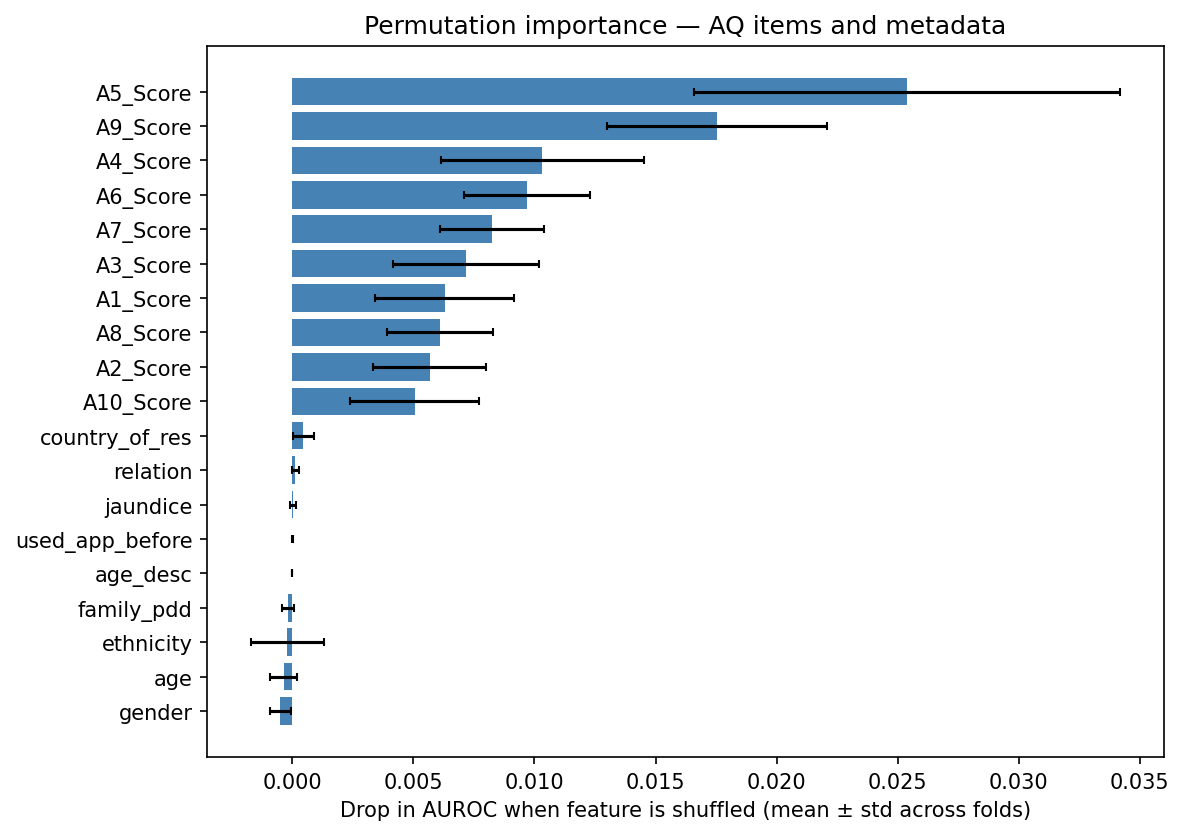
\includegraphics[width=0.82\linewidth]{imagens/rf_permutation_importance.png}
    }{%
      \textcolor{gray}{\small [Ejecutar celda 2 del cuaderno para generar \texttt{imagens/rf\_permutation\_importance.png}]}
    }
  \end{center}
  \vspace{-0.3em}
  {\tiny Cada barra = caída media en AUROC al permutar esa variable; barras de error = desviación estándar entre folds.
  Variables con barra larga son las más decisivas para la clasificación.}
\end{frame}

\begin{frame}{Ética, limitaciones y aportes previstos}
  \begin{itemize}
    \setlength{\itemsep}{0.25em}
    \footnotesize
    \item \textbf{Ética:} anonimización, consentimiento; fines de \emph{screening} preliminar, no diagnóstico.
    \item \textbf{Limitaciones:} sesgos de muestreo, representatividad; hace falta validación clínica y externa.
    \item \textbf{Aportes:} constatar que no todos los ítems pesan igual; subconjuntos con desempeño similar; explicaciones comprensibles para triage; sin confundir puntaje o probabilidad con verdad clínica.
  \end{itemize}
\end{frame}

\begin{frame}{Justificación (puente hacia el cuaderno)}
  Sobre UCI-426, el cuaderno entrena un modelo con ítems y metadatos, validación cruzada, importancia de variables, y análisis de regla fija, forma corta, \emph{clusters} y \textbf{equidad}---siempre con transparencia sobre correlaciones, tamaño $n$ y riesgo de sesgo, coherente con el planteamiento de \texttt{prop.tex} y con el repositorio del proyecto.
\end{frame}

% -------------------------------------------------------------------------
\section{Recursos}

\begin{frame}{Repositorio, datos y cuestionario oficial}
  \begin{itemize}
    \setlength{\itemsep}{0.45em}
    \item Código, notebook, documentación: \url{https://github.com/ebooshi/DIAA-Proyecto-2026}
    \item Conjunto: \href{https://archive.ics.uci.edu/dataset/426/autism+screening+adult}{Autism Screening Adult} (id 426, DOI \href{https://doi.org/10.24432/C5F019}{10.24432/C5F019}).
    \item AQ-10 (adultos, PDF de referencia): \href{https://leademployer.merseywestlancs.nhs.uk/media/Neurodiversity/Adult-autism-AQ10-questionnaire-test-v1.pdf}{versión en línea}.
  \end{itemize}
\end{frame}

\begin{frame}{Notas técnicas (placeholders del cuaderno)}
  \begin{itemize}
    \setlength{\itemsep}{0.35em}
    \footnotesize
    \item Limpieza, codificación; objetivo: etiqueta binaria; \texttt{result} excluido de predictores en el hilo de modelado.
    \item \textbf{Modelo:} p.\,ej.\ bosque aleatorio con \texttt{Pipeline}, CV estratificada, importancia y equidad.
    \item Sustituir esta diapositiva con figuras por cada bloque (ítems, regla, reducción, clusters, subgrupos).
  \end{itemize}
\end{frame}

\begin{frame}[t,allowframebreaks]{Referencias}
  \scriptsize
  \begin{thebibliography}{99}
    \bibitem{towle2016}
    Towle P, Patrick P. Instrumentos de tamizaje de TEA en edades muy tempranas: revisión sistemática. New York: Hindawi, 2016.
    \bibitem{cdc2014}
    Centers for Disease Control and Prevention. Prevalencia de TEA (8 años, 11 sitios, EE.\,UU., 2010). \emph{MMWR} 2014; 63(2): 1--21.
    \bibitem{lord1994}
    Lord C, Rutter M, Le~Couteur A. \emph{Autism Diagnostic Interview-Revised}. J Autism Dev Disord 1994; 24: 659--685.
    \bibitem{lord2000}
    Lord C, Risi S, Lambrecht L, et~al. \emph{ADOS-Generic}. J Autism Dev Disord 2000; 30: 205--223.
    \bibitem{fitzgerald2017}
    Fitzgerald M. Gestalts clínicos del autismo. In: Fitzgerald M, Yip~J (eds). \emph{Autism: paradigms, recent research and clinical applications.} Rijeka: InTech, 2017: 1--13.
    \bibitem{crane2016}
    Crane L, Chester J, Goddard~L, et~al. Experiencias con el diagnóstico de TEA: encuesta a padres. \emph{Autism} 2016; 20(2): 153--162.
    \bibitem{thabtah2020}
    Thabtah F, Peebles~D. Un modelo de inducción de reglas para detección de TEA. \emph{Health Informatics Journal} 2020, 26(1): 264--286. \url{https://journals.sagepub.com/doi/10.1177/1460458219866030}
    \bibitem{aq10pdf}
    Cuestionario AQ-10 (adultos), versión PDF. Mersey / NHS. \url{https://leademployer.merseywestlancs.nhs.uk/media/Neurodiversity/Adult-autism-AQ10-questionnaire-test-v1.pdf}
    \bibitem{apoyo_tea}
    Material de apoyo: ADI, ADOS, literatura de tamizaje y ML en psicometría (ampliar en memoria o tesis).
    \bibitem{uci426}
    Thabtah~F. (creador). \emph{Autism Screening Adult.} UCI Machine Learning Repository (ID~426), 2017. DOI: \href{https://doi.org/10.24432/C5F019}{10.24432/C5F019}. \url{https://archive.ics.uci.edu/dataset/426/autism+screening+adult}
    \bibitem{gh_repo}
    \emph{DIAA--Proyecto 2026} (repositorio: código, notebook, documentación). GitHub, 2026. \url{https://github.com/ebooshi/DIAA-Proyecto-2026}
  \end{thebibliography}
\end{frame}

\end{document}
